\begin{figure}[ht]
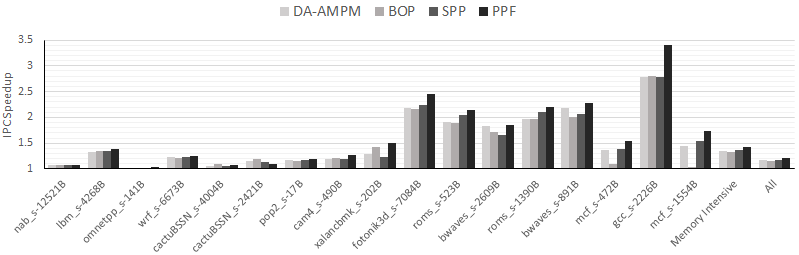
\includegraphics[width=\columnwidth]{SPEC2017}
\caption{SPEC CPU 2017 Single-Core IPC Speedup}
\label{Fig:SPEC2017_1core}
\end{figure}

\section{Results}
\label{Results}

This section discusses the results obtained from running PPF in terms of
prefetch cache coverage and speedup. For the SPEC CPU 2017 benchmarks, first
we present the results for single-threaded workloads then for multi-core
workloads.

\subsection{Single-core Results}
\label{Results-Single}

% djimenez: why is this figure described this way? it's not OK to just
% highlight noticeable improvement. the benchmarks must be selected by some
% unbiased criteria, e.g. some minimum MPKI under LRU or some minimum speedup
% under a baseline prefetcher that isn't PPF.

Figure~\ref{Fig:SPEC2017_1core} shows the IPC speedup obtained by PPF,
compared to BOP, DA-AMPM and SPP; for the individual SPEC CPU 2017 
applications, followed by memory intensive subset and finally the full
suite. All the results have been normalized to the baseline of no prefetching.

% djimenez: you've inconsistently italicized and not italicized benchmark
% names. i'll help you out here; i like putting them in a typewriter font so
% i'll do that throughout this section. also, you've inconsistent put and not put
% the number of the benchmark. i'll fix that too.

PPF yields a geometric mean speedup of \textbf{26.95\%} over the baseline. 
This is equivalent to \textbf{4.63\%} over DA-AMPM, \textbf{4.61\%} over BOP 
and \textbf{3.78\%} over SPP. Out of the 95 simpoints developed for SPEC 
CPU 2017, PPF nearly matches or outperforms most of the prefetchers on 91 
simpoints. PPF fails to match the improvement offered by BOP only for 
{\tt 607.cactuBSSN\_s} and {\tt 654.roms\_s} traces.

At its peak, PPF manages a speedup of a factor of over \textbf{3.39x} on one of the
{\tt 602.gcc\_s} traces. This also corresponds to speedup gain of
\textbf{60\%} over the next best prefetcher for that trace -- BOP. In general, benchmarks
{\tt 603.bwaves\_s}, {\tt 605.mcf\_s}, {\tt 623. xalancbmk\_s} and {\tt
649.fotonik3d\_s} benefit the most from PPF, with the speedup over SPP ranging
from \textbf{10\% to 25\%}.

% djimenez: is this geometric mean? if so, say so.
% [EB] Resolved
On the full SPEC CPU 2017 suite, PPF improves the geometric mean IPC of 
the baseline by \textbf{15.24\%}, which is \textbf{2.27\%} better 
than the next best prefetcher -- SPP.
\newline

\begin{figure}[h]
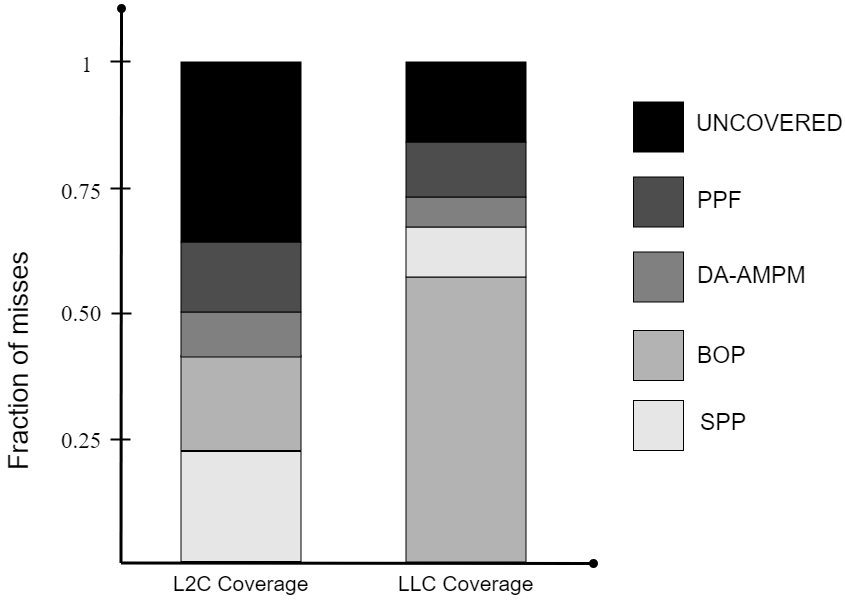
\includegraphics[width=\columnwidth]{Coverage}
\caption{Fraction of Cache Misses Covered}
\label{Fig:Coverage}
\end{figure}

% djimenez: this is a weird way to make a header for a section. use \paragraph or \subsection

\noindent \textbf{COVERAGE}
\newline
Prefetcher coverage is defined as the ratio of the number of misses avoided
through prefetching to the number of misses with no prefetching.

Figure~\ref{Fig:Coverage} shows the fraction of misses in the L2 and LLC
avoided by the various prefetchers. PPF has the highest coverage of all the
prefetchers simulated. On the SPEC CPU 2017 benchmarks, PPF reduces misses by
\textbf{62.5\%} and \textbf{82.8\%} in the L2 and LLC respectively. For the
same benchmark, the next best prefetcher, DA-AMPM, covers \textbf{48.6\%} and
\textbf{72.8\%} of the misses respectively.

This superior coverage of PPF can be attributed to aggressive re-tuning of the
underlying SPP, enabled by the Perceptron Filter making sure the high coverage
does not lead to increased cache pollution.

%\begin{figure*}[ht]
%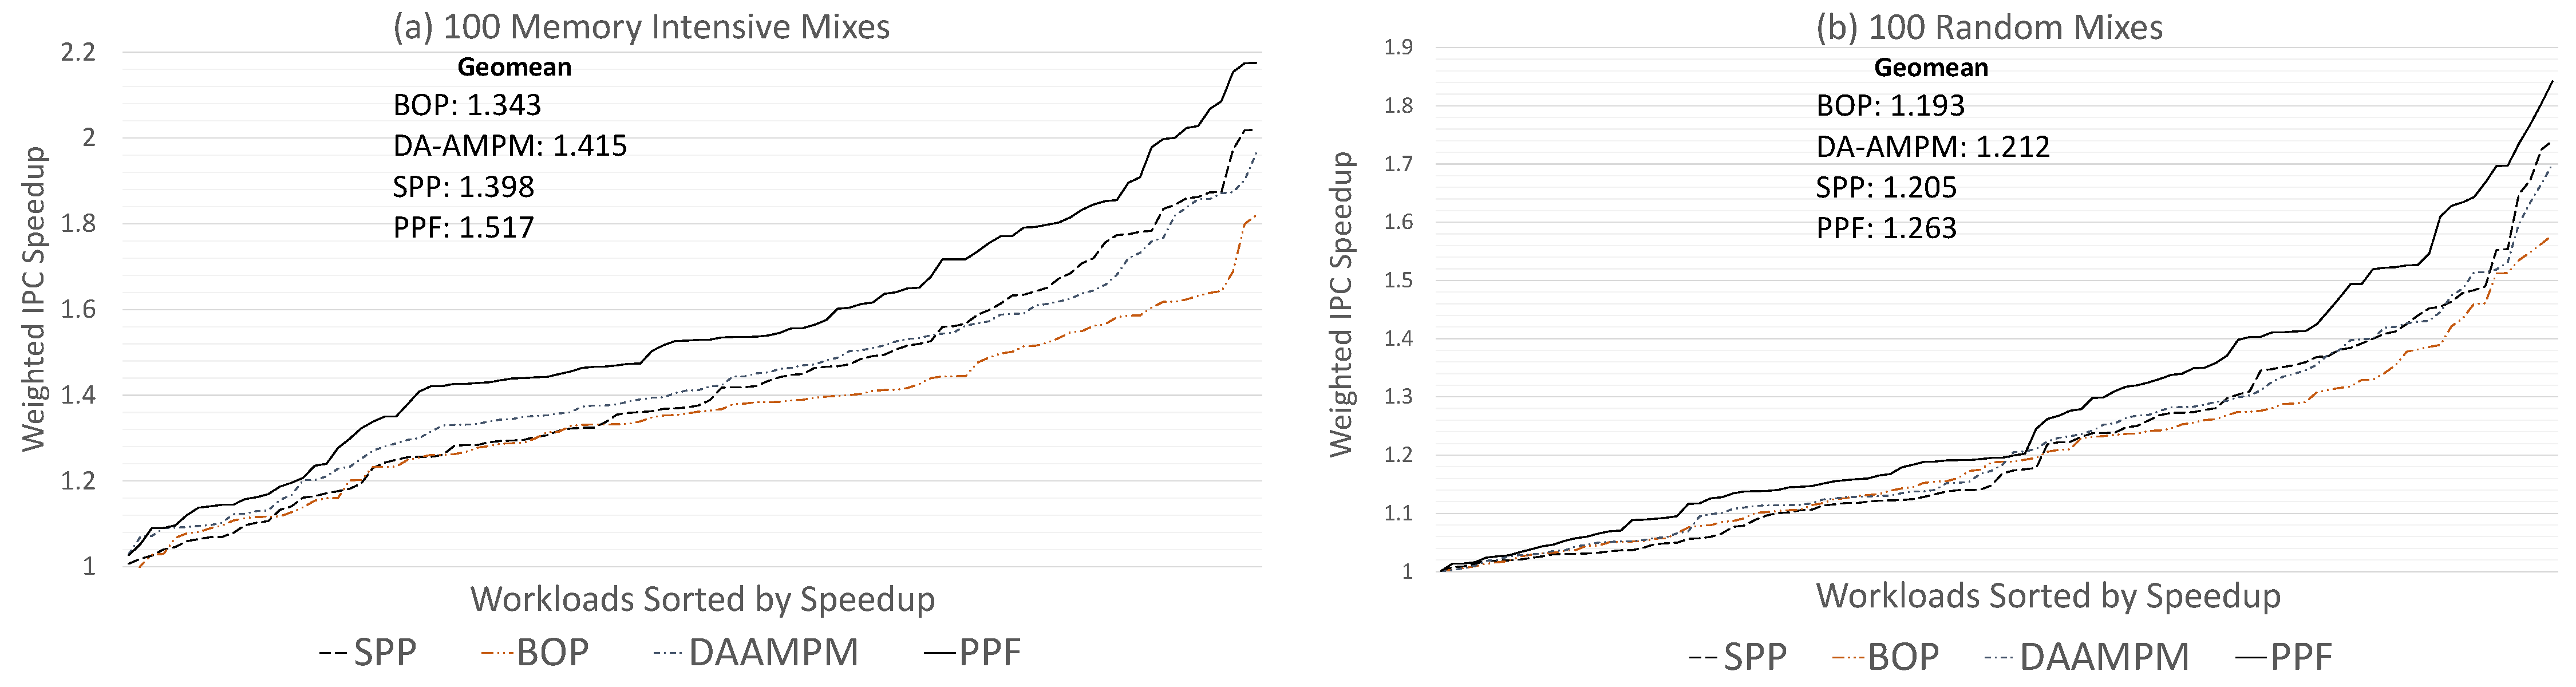
\includegraphics[width=\textwidth]{4Core_SPEC2017}
%\caption{Normalized Speedup for 4-core SPEC CPU 2017 Workloads}
%\label{Fig:4Core_SPEC2017}
%\end{figure*}

\begin{figure}[ht]
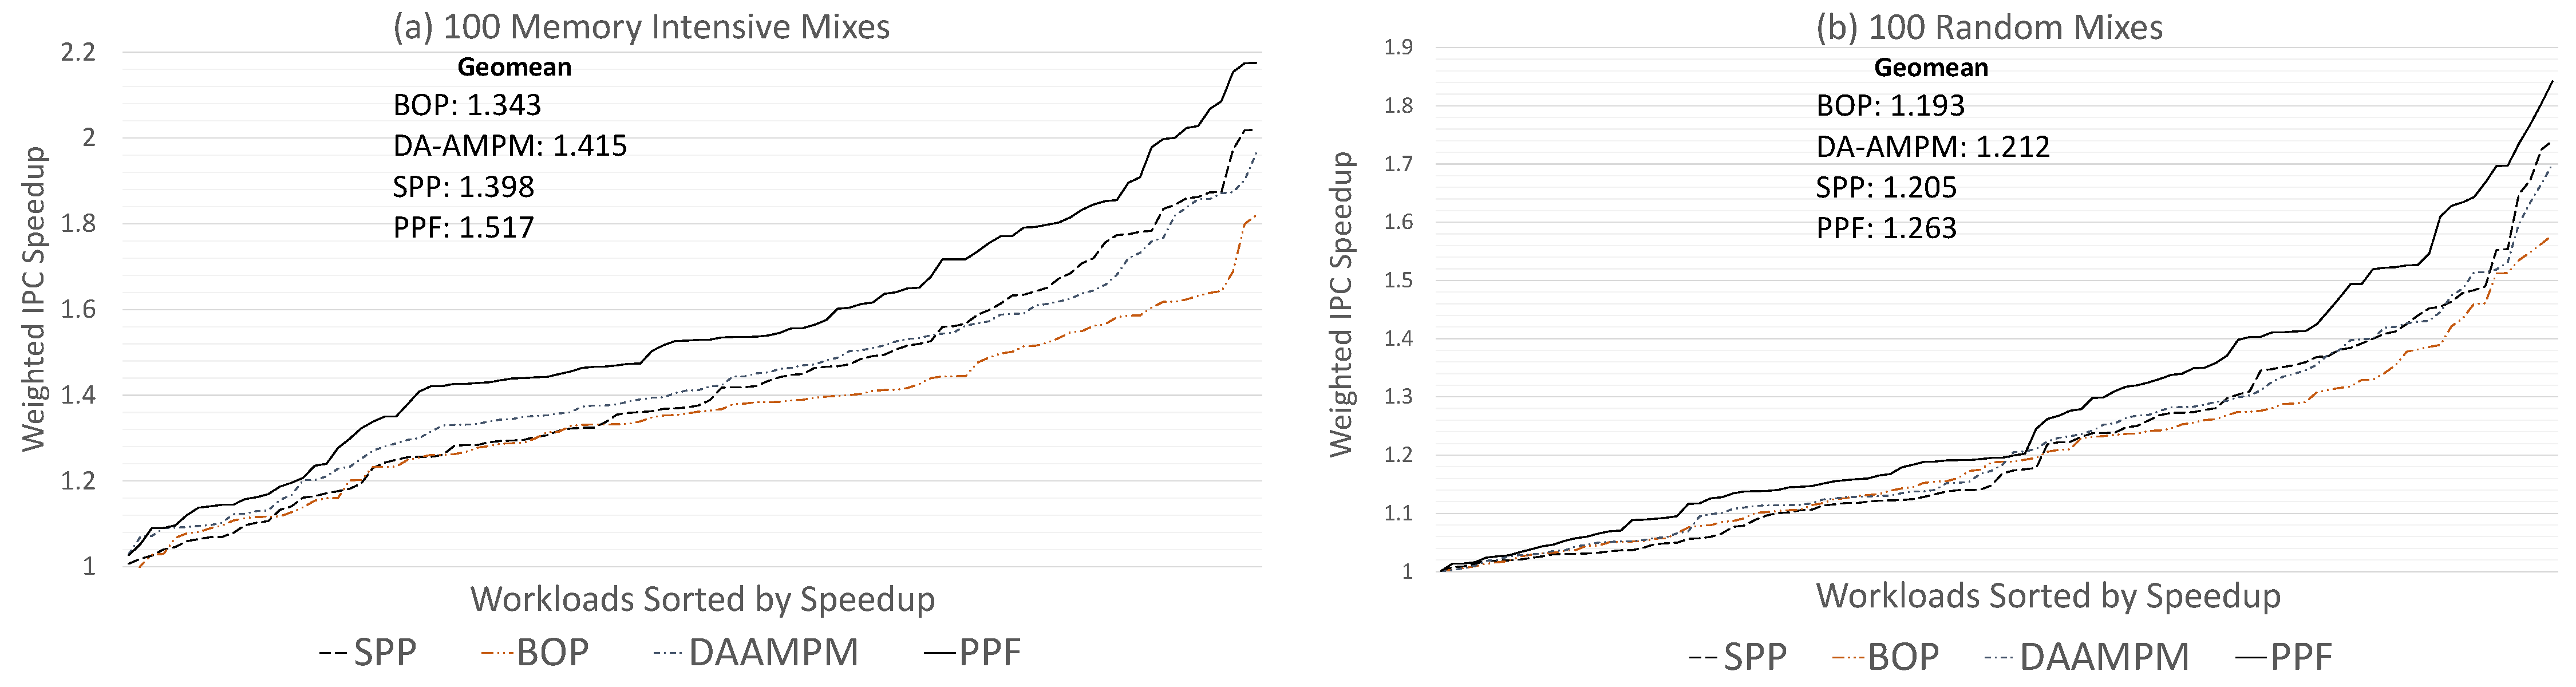
\includegraphics[width=2.75in]{4Core_SPEC2017}
\caption{Speedup for 4-core SPEC CPU 2017}
\label{Fig:4Core_SPEC2017}
\end{figure}

\subsection{Multi-core Results}
\label{Results-Multi}
In this section, we demonstrate the improvement achieved by PPF for a mix of
multi-programmed workloads.
\newline

\noindent \textbf{4-CORE ENVIRONMENT}
\newline
Figure~\ref{Fig:4Core_SPEC2017} shows a comparison of speedups obtained on
4-core mixes of a memory intensive subset SPEC CPU 2017. We plot all 4
prefetchers, normalized to the baseline. The workloads have been sorted in
increasing order of the speedup. PPF offers a speedup of \textbf{51.2\%} on
these traces, and improvement of \textbf{11.4\%} over the baseline SPP,
\textbf{9.7\%} over the next DA-AMPM, and \textbf{16.9\%} over BOP.

On a different set of fully random SPEC CPU 2017 4-core mixes (not illustrated
for space reasons), PPF provides an IPC speedup of \textbf{26.07}\% over the
baseline, which is an improvement of \textbf{5.6}\% over SPP.

%\begin{figure*}[ht]
%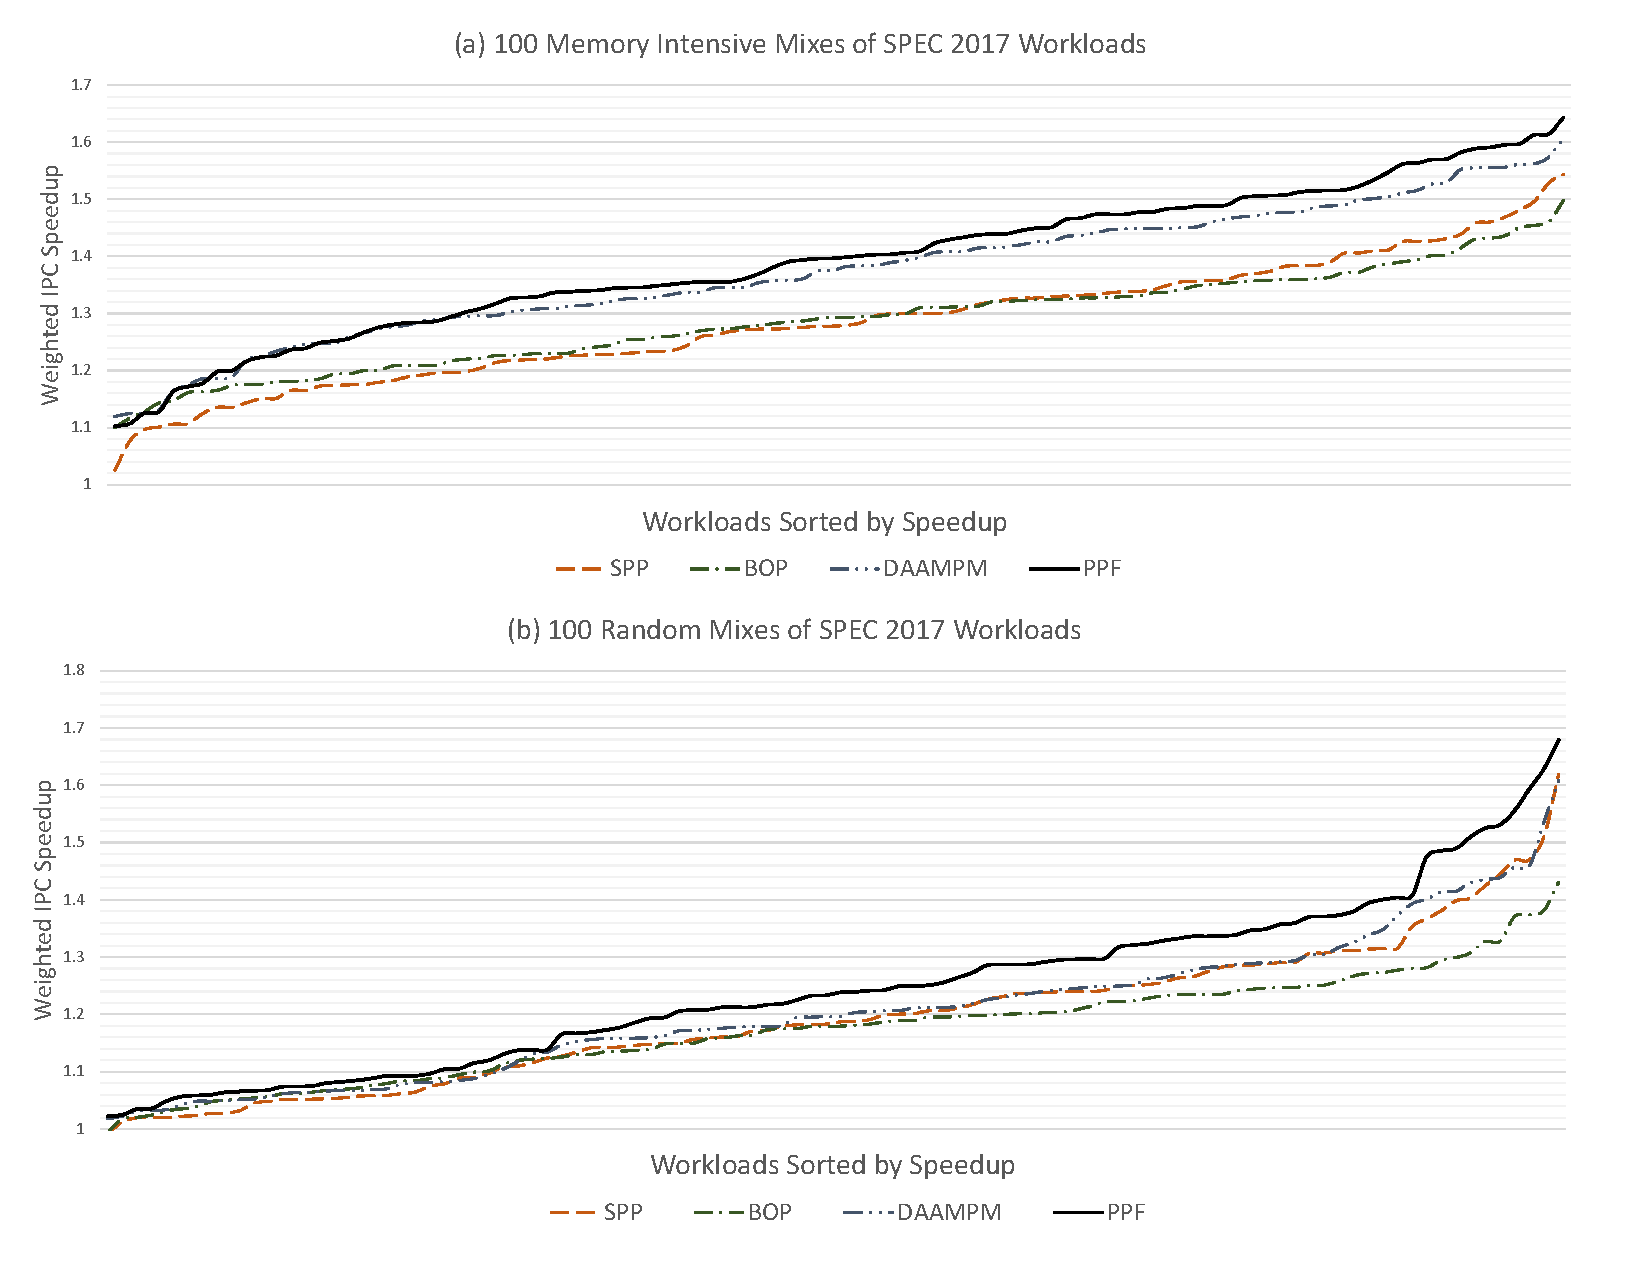
\includegraphics[width=\textwidth]{8Core_SPEC2017}
%\caption{Normalized Speedup for 8-core SPEC CPU 2017 Workloads}
%\label{Fig:8Core_SPEC2017}
%\end{figure*}

\begin{figure}[ht]
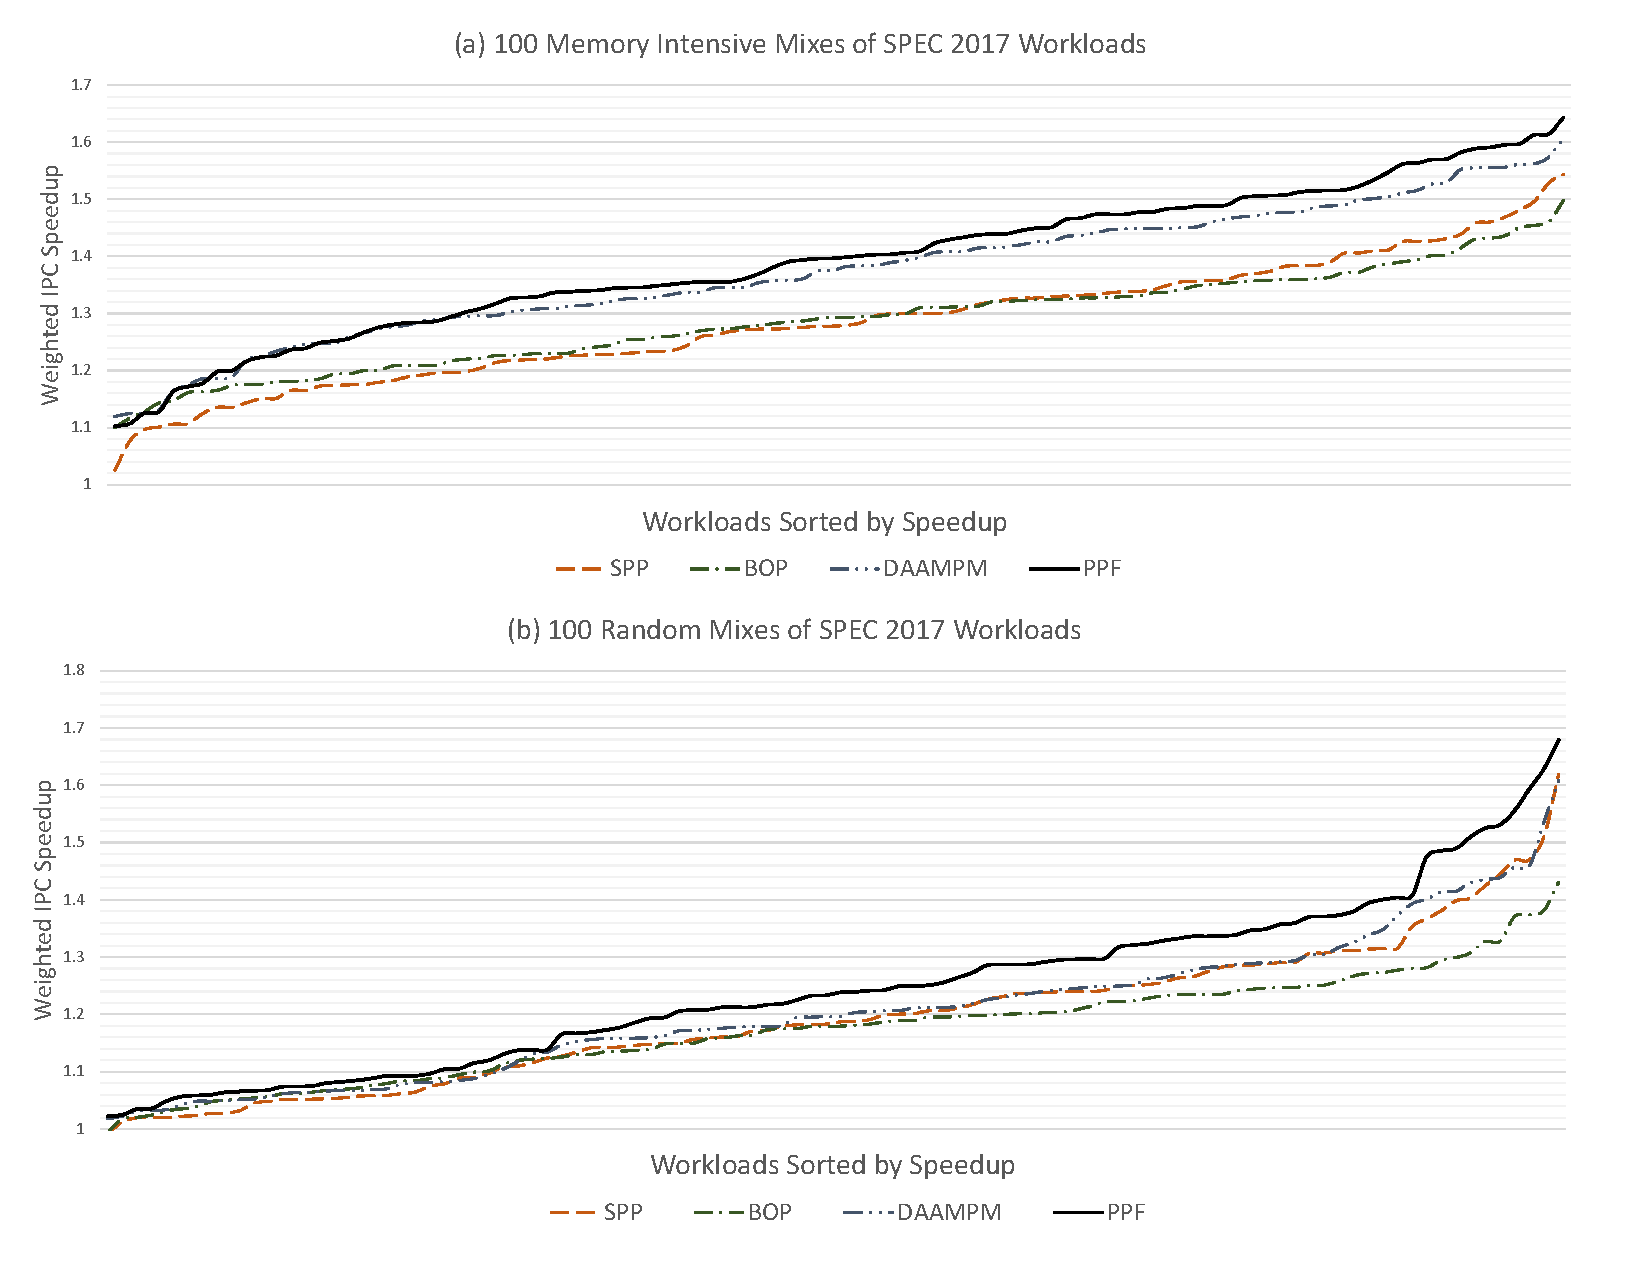
\includegraphics[width=2.75in]{8Core_SPEC2017}
\caption{Speedup for 8-core SPEC CPU 2017}
\label{Fig:8Core_SPEC2017}
\end{figure}

\noindent \textbf{8-CORE ENVIRONMENT}
\newline
The sorted comparison of speedups on the memory intensive 8-core mixes is
shown in Figure~\ref{Fig:8Core_SPEC2017}. PPF improves baseline performance
by \textbf{37.6\%}, an improvement of \textbf{9.7\%} over SPP. For a random
set of SPEC CPU 2017 mixes (not illustrated for space reasons), PPF improves
performance by \textbf{23.4\%} over the baseline, corresponding to
\textbf{4.6\%} over SPP. This increased improvement achieved by PPF over the
base engine SPP in a multi-core environment is expected as PPF has a very
accurate filter, it eliminates useless prefetches before they can cause
pollution in the shared LLC.

BOP offers a better improvement than SPP for the memory intensive mixes. This
superiority can be attributed to BOP's inherent aggressive nature. DA-AMPM is
also ahead of SPP in both the mixes. Interestingly, in all these cases, PPF
consistently outperforms the best performing prefetcher.

% djimenez: cut this graph and modified text accordingly
%\begin{figure}[ht]
%\begin{adjustwidth}{-1cm}{}
%  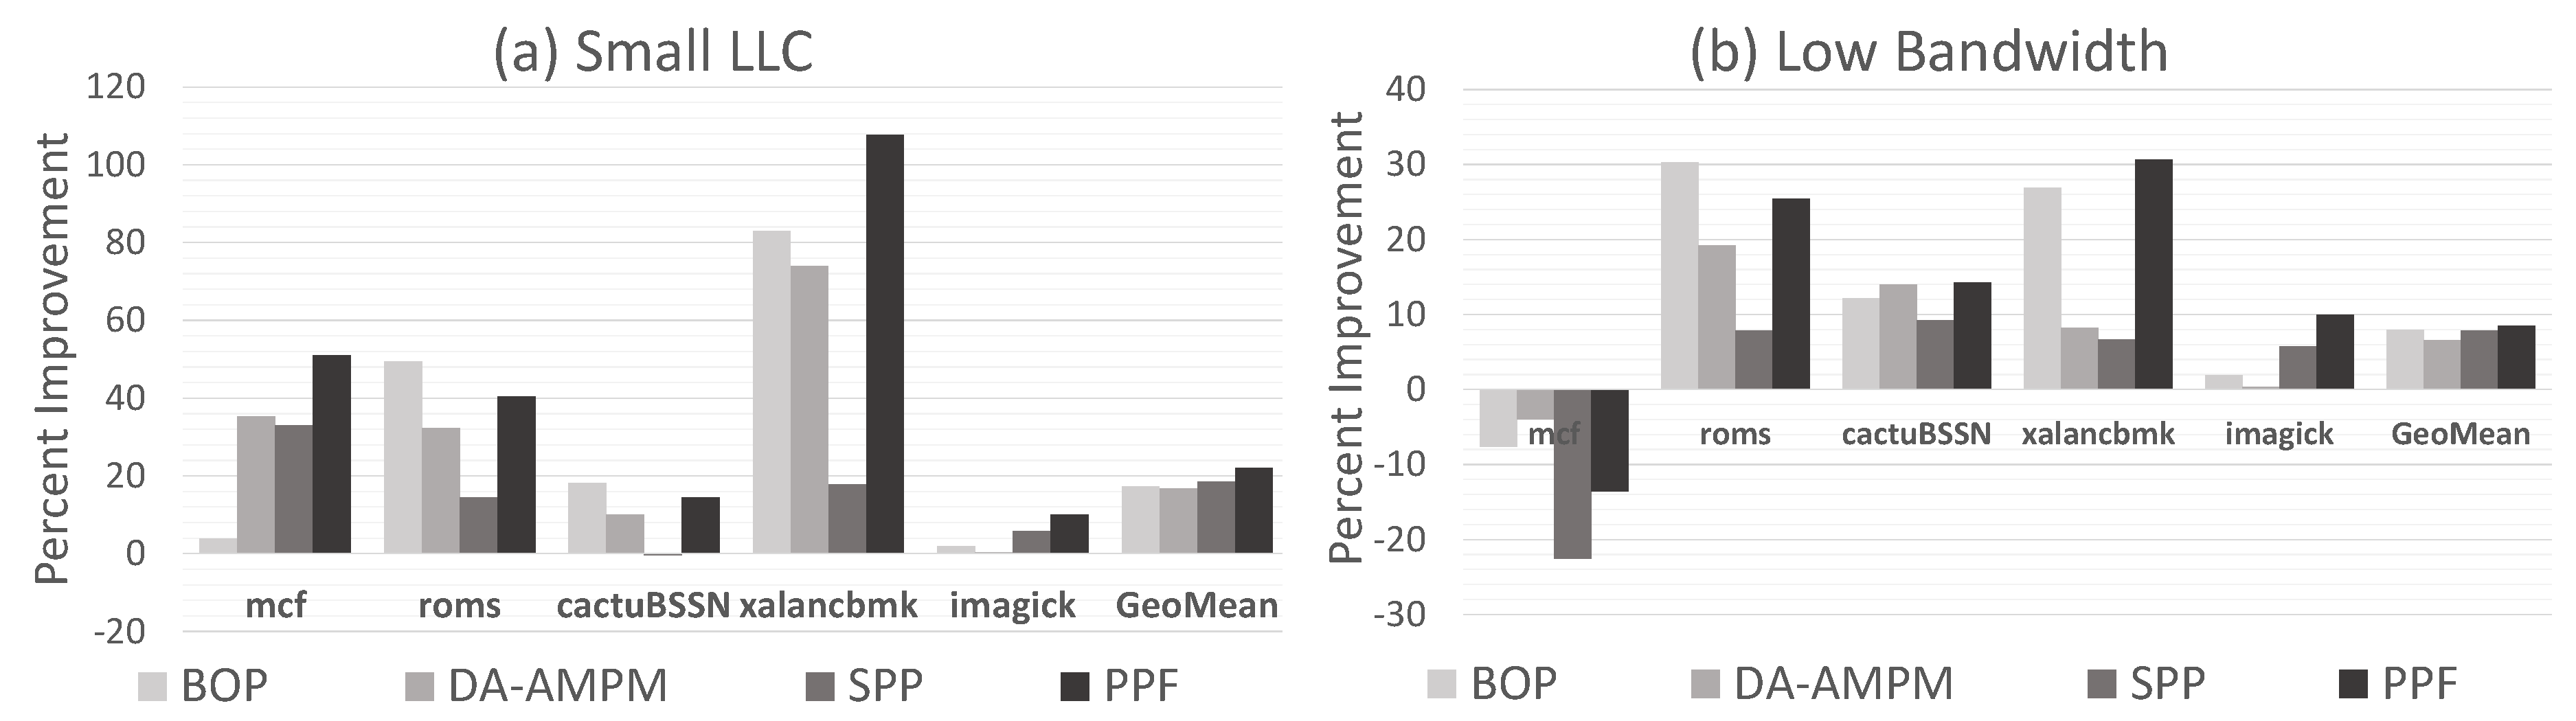
\includegraphics[width=1.2\columnwidth]{AddnConstr}
%  \caption{IPC speedup for Small LLC and Low BW}
%  \label{Fig:AddnConstr}
%\end{adjustwidth}
%\end{figure}

\subsection{Additional Memory Constraints}
\label{Results-AdditionalMem}

%Figure~\ref{Fig:AddnConstr}(a) and (b) show the performance of PPF in a
%followed by the overall performance on the complete benchmark.  
%For the sake of brevity, we have only shown selected traces 

We also model PPF with reduced LLC and with low bandwidth constraints,
respectively (not illustrated for space reasons). Benchmark {\tt 605.mcf\_s}
in low bandwidth conditions is prefetch averse. In general, any prefetcher
yields a negative speedup on that trace. On {\tt 654.roms\_s} and {\tt
607.cactuBSSN\_s}, PPF is unable to match the performance achieved by the best
prefetcher. On the other hand, PPF outperforms all the other prefetchers on
{\tt 623.xalancbmk\_s} and {\tt 638.imagick\_s} benchmarks. Overall, PPF
gives a better improvement under small LLC condition and matches the best
prefetcher, BOP, under low DRAM bandwidth conditions.

\begin{figure}[ht]
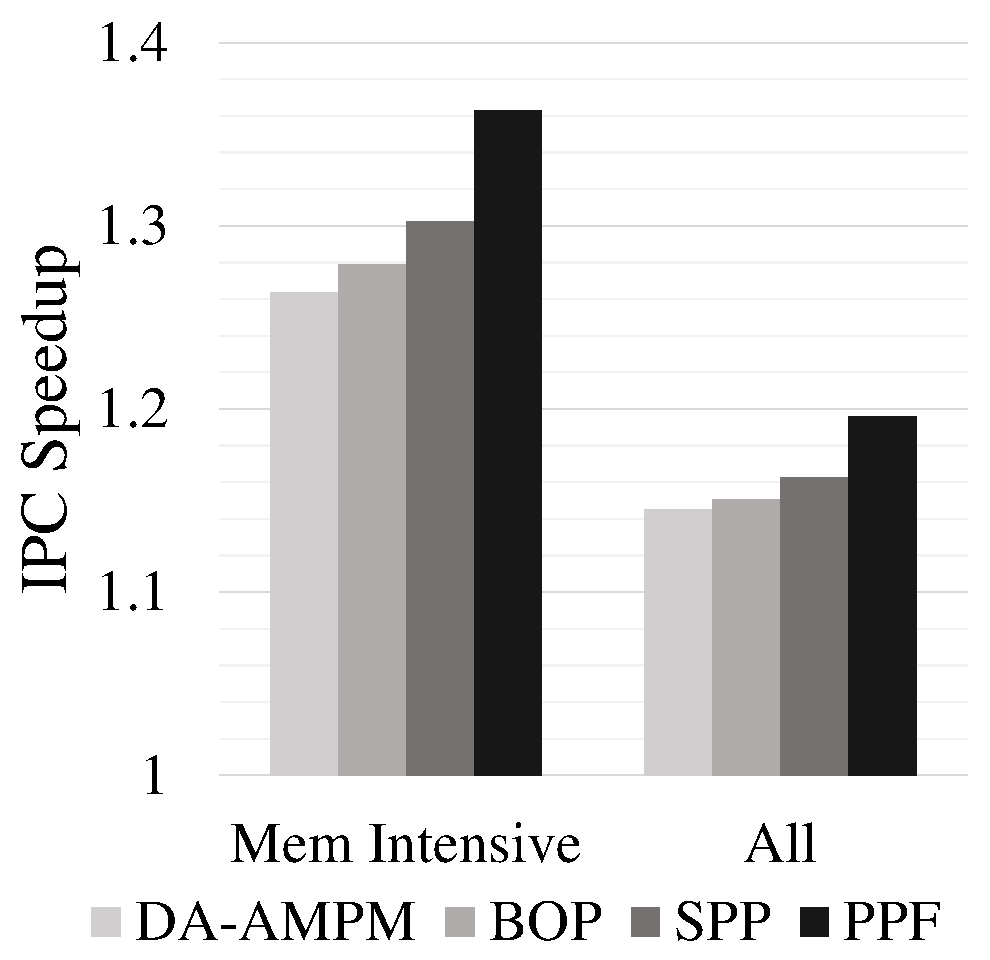
\includegraphics[width=\columnwidth]{SPEC2006}
\caption{SPEC CPU 2006 Single-Core IPC Speedup}
\label{Fig:SPEC2006_1core}
\end{figure}

\begin{figure}[ht]
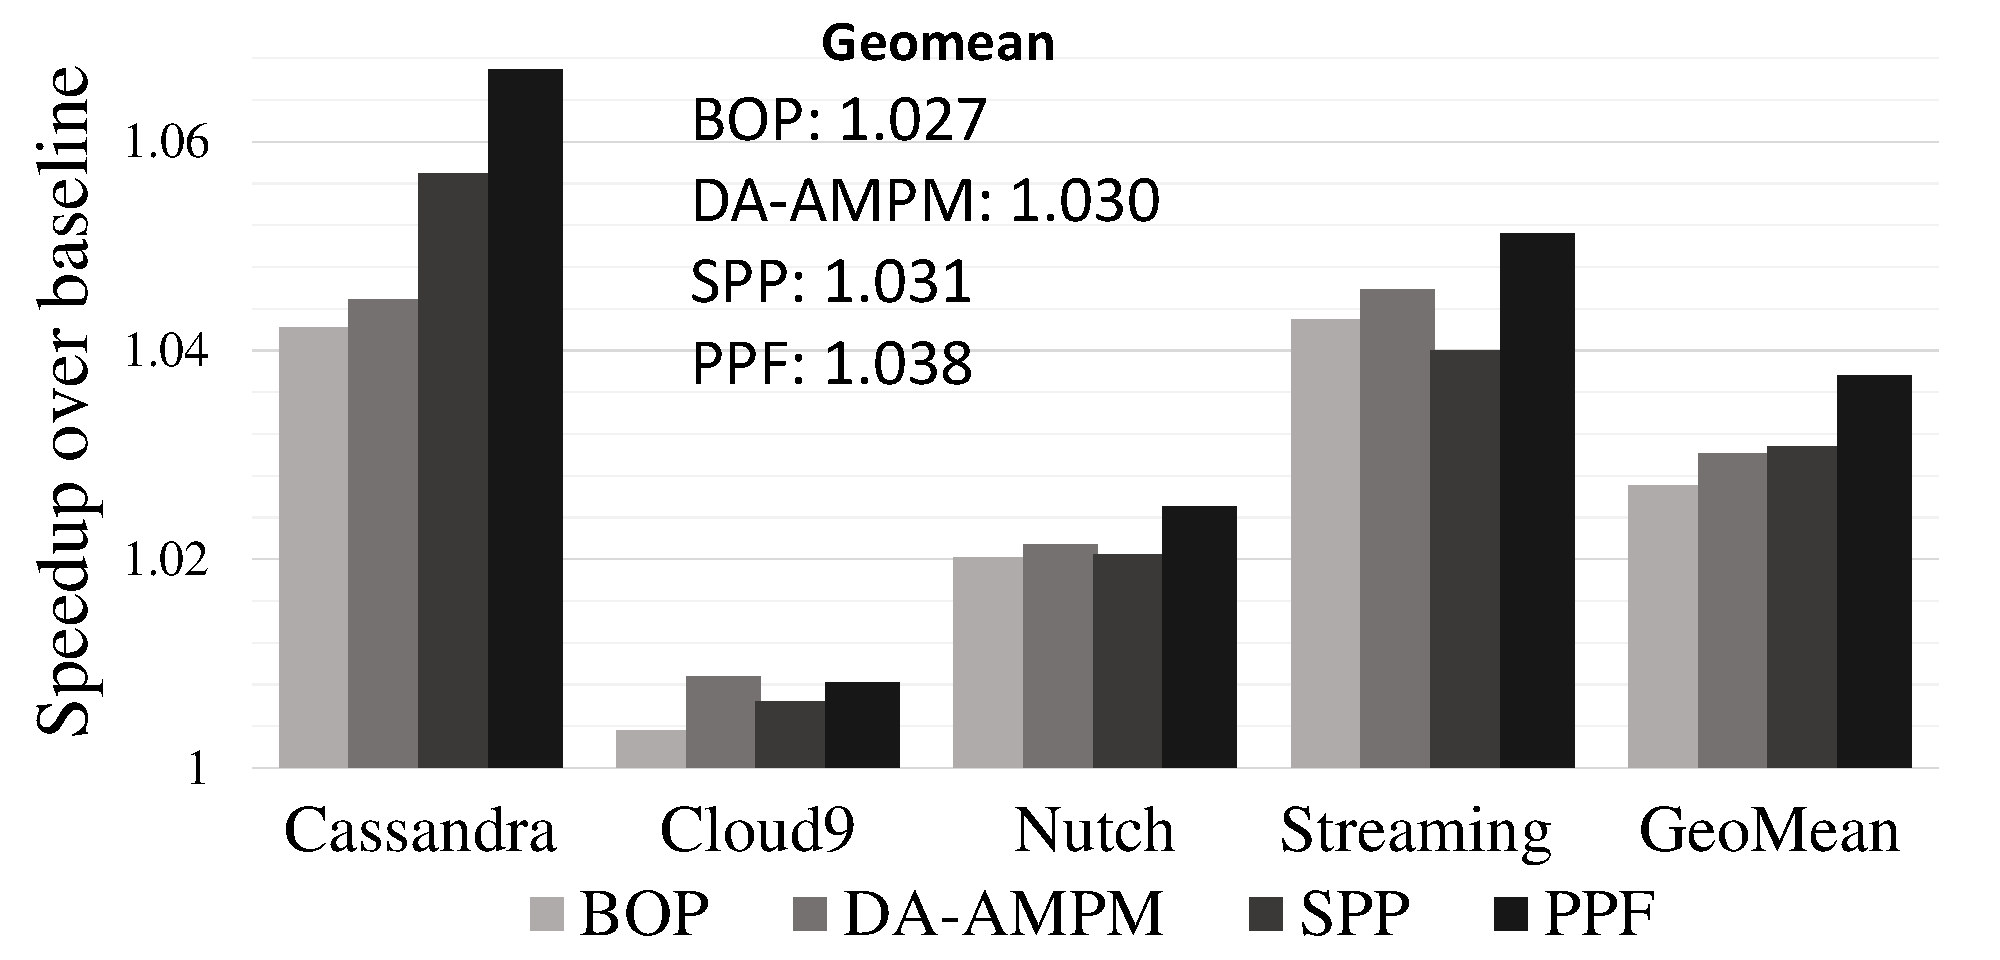
\includegraphics[width=\columnwidth,]{CloudSuite}
\caption{IPC Speedup for Multi-core CloudSuite Workloads}
\label{Fig:CloudSuite}
\end{figure}

\subsection{Cross Validation}
\label{Results-CrossVal}

% djimenez: cite cloudsuite here? do we have a reference?
% [EB]: Resolved. Cited "Clearing the clouds: A study of emerging 
%        scale-out workloads on modern hardware" in methodology

Here we demonstrate the robustness of PPF by testing it on different
benchmarks: SPEC CPU 2006 and CloudSuite.

% djimenez: is the improvement over BOP and DA-AMPM exactly the same 9.86%
% here? that's weird.
% [EB] Resolved. Increased precision of values. But yes, BOP / DA-AMPM 
% have really close numbers for SPEC 2006

Figure~\ref{Fig:SPEC2006_1core} shows the speed-up achieved by BOP, SPP and
PPF on the memory intensive subset and the full SPEC CPU 2006 suite. 
PPF provides a speedup of \textbf{36.3\%} over the baseline on the 
memory intensive subset of SPEC CPU
2006 benchmark, giving an improvement of \textbf{6.1\%} over SPP and
\textbf{8.44\%} over DA-AMPM and \textbf{9.93} over BOP. On the whole of 
the SPEC CPU 2006 suite, the speedup is \textbf{19.6\%}, an improvement 
of \textbf{3.33\%} over SPP.

For 4-core memory intensive mixes, PPF improves the baseline by
\textbf{59.1\%}, \textbf{8.6\%} ahead of SPP. For 8-core memory intensive
mixes, the speedup over the baseline is \textbf{47.8\%}, \textbf{11.3\%} ahead
of SPP.

Figure~\ref{Fig:CloudSuite} shows the performance benefit comparison of all
the prefetch schemes on 4 different applications in the CloudSuite benchmark.
In general, these applications are prefetch agnostic. Even so, PPF manages a
\textbf{3.78\%} improvement over no prefetching, putting it ahead of the next
best prefetcher, SPP, which provides a 3.08\% speedup.

We developed PPF to yield good performance on the SPEC CPU 2017 benchmarks.
Nevertheless, the performance is consistently good on other benchmark suites.
We attribute this fact to the inherent adaptability of the perceptron model.
In general, perceptron weights are able to adjust in real-time so as to find
the best possible correlation between the output and the given set of
features.
